%*****************************************
\chapter{Unobtrusive Research}\label{ch12:unobtrusive}
%*****************************************
% Blackstone p 137
% Covers content analysis and secondary research
% Add something about meta-analysis???
%TODO Status: Pre-draft

\section{Introduction}

\begin{wrapfigure}{r}{0.4\textwidth}
	\centering
	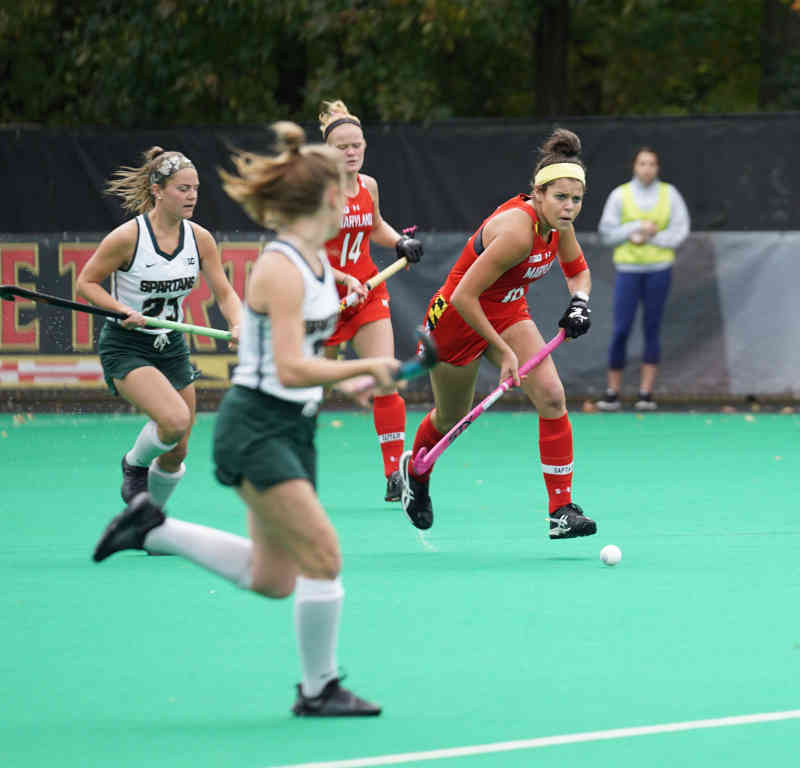
\includegraphics[width=0.4\textwidth]{gfx/12-women_hockey} 
\end{wrapfigure}

Are female and male athletes at the professional and college levels treated equally? It would be reasonable to think, 40 years since the passing of Title IX (the civil rights law that prohibits sex discrimination in education including athletics) and with the growing visibility of women athletes in sports such as golf, basketball, hockey, and tennis, that the answer would be an easy yes. But Professor Michael Messner's \cite{messner2002taking} unobtrusive research shows otherwise, as does Professors Jo Ann M. Buysse and Melissa Sheridan Embser-Herbert's \cite{buysse2004constructions} content analysis of college athletics media guide photographs. In fact, Buysse and Embser-Herbert's unobtrusive research shows that traditional definitions of femininity are fiercely maintained through colleges' visual representations of women athletes as passive and overtly feminine (as opposed to strong and athletic). Unobtrusive research made it possible to clear up misconceptions about changes for women athletes over the past 40 years.\blfootnote{Photo by Jeffrey F Lin on Unsplash}

\begin{center}
	\begin{objbox}{Objectives}
		\begin{itemize}
			\setlength{\itemsep}{0pt}
			\setlength{\parskip}{0pt}
			\setlength{\parsep}{0pt}
			
			\item Define ``Unobtrusive Research.''
			\item Describe the strengths and weaknesses of unobtrusive research.
			\item Describe methods used for unobtrusive data collection and analysis.
			\item Describe how data collected by others can be used.
			\item Discuss reliability in unobtrusive research.
		\end{itemize}
	\end{objbox}
\end{center}

\section{What Is Unobtrusive Research?}

This chapter explores unobtrusive methods of collecting data, which are methods that do not interfere with the subjects under study. Both qualitative and quantitative researchers use unobtrusive research methods. Unobtrusive methods share the unique quality that they do not require researchers to interact with the people they are studying. It may seem strange that business, a discipline dedicated to understanding human purchasing behavior, would employ a methodology that requires no interaction with human beings. But humans create plenty of evidence of their behaviors---they write letters to the editor of their local paper, they create various sources of entertainment for themselves such as movies and televisions shows, they consume goods, they walk on sidewalks, they lie on the grass in public parks. All these activities leave something behind---worn paths, trash, recorded shows, and printed papers. These are all potential sources of data for the unobtrusive researcher.

Unobtrusive research methods include content analysis, indirect measures, and data collected by others. All of these methods are similar in that they do not require direct interaction between researchers and their human subjects but each has its unique qualities. This chapter also considers how data gathered unobtrusively can be analyzed and how reliability can be improved.

\subsection{Strengths of Unobtrusive Research}

Researchers who seek evidence of what people actually do, as opposed to what they say they do (as in survey and interview research), might wish to consider using unobtrusive methods. Field researchers may also claim this advantage over interview and survey research, but field researchers cannot be certain about what effect their presence in the field may have on the people and the interactions that they observe. While unobtrusive research projects, like all research projects, face the risk of introducing researcher bias into the work, researchers employing unobtrusive methods do not need to be concerned about the effect of the research on their subjects. This effect, known as the \gls{hawthorne}, is not a concern for unobtrusive researchers because they do not interact directly with their research participants. In fact, this is one of the major strengths of unobtrusive research.
%TODO Start Here
Another benefit of unobtrusive research is that it can be relatively low-cost compared to some of the other research methods. Because ``participants'' are generally inanimate objects as opposed to human beings, researchers may be able to access data without having to worry about paying participants for their time (though certainly travel to or access to some documents and archives can be costly).

Unobtrusive research is also relatively forgiving. It is far easier to correct mistakes made in data collection when conducting unobtrusive research than when using any other method. Imagine the challenge, for example, if researchers realized at the end of conducting 50 in-depth interviews that they had accidentally omitted two critical questions from the interview guide. What options would they have? Reinterview all 50 participants? Try to figure out what they might have said based on their other responses? Reframe the research question? Scratch the project entirely? Obviously none of these options is ideal. The same problems arise if a mistake is made in survey research. For field researchers, the consequences of ``messing up'' during data collection can be even more disastrous. Imagine discovering after tagging along on a political candidate's campaign that a ``do-over'' is needed. In this case, that simply is not an option. The campaign is over, and the researcher would need to find a new source of data. Fortunately for unobtrusive researchers, going back to the source of the data to gather more information or correct some problem in the original data collection is a relatively straightforward prospect.

Finally, unobtrusive research is well suited to studies that focus on processes that occur over time. While longitudinal surveys and long-term field observations are also suitable ways of gathering such information, they cannot examine processes that occurred decades before data collection began, nor are they the most cost-effective ways to examine long-ranging processes. Unobtrusive methods, on the other hand, enable researchers to investigate events and processes that have long since passed. They also do not rely on retrospective accounts, which may be subject to errors in memory, as some longitudinal surveys do.

In sum, the strengths of unobtrusive research include the following:

\begin{enumerate}
	\item There is no possibility for the Hawthorne effect.
	\item The method is cost effective
	\item It is easier in unobtrusive research than with other methods to correct mistakes.
	\item Unobtrusive methods are conducive to examining processes that occur over time or in the 
\end{enumerate}past.

\subsection{Weaknesses of Unobtrusive Research}

While there are many benefits to unobtrusive research, this method also comes with a unique set of drawbacks. Because unobtrusive researchers analyze data that may have been created or gathered for purposes entirely different from the researcher's goal, problems of validity sometimes arise in such projects. It may also be the case that data sources measuring whatever a researcher wishes to examine simply do not exist. This means that unobtrusive researchers may be forced to tweak their original research interests or questions to better suit the data that are available to them. Finally, it can be difficult in unobtrusive research projects to account for context. In a field research project, for example, the researcher is able to see what events lead up to some occurrence and observe how people respond to that occurrence. What this means for unobtrusive research is that while it can be difficult to ascertain why something occurred, we can gain a good understanding of what has occurred.

In sum, the weaknesses of unobtrusive research include the following:

\begin{enumerate}
	\item There may be potential problems with validity.
	\item The topics or questions that can be investigated are limited by data availability.
	\item It can be difficult to see or account for social context.
\end{enumerate}

\section{Unobtrusive Data Collection}

This section focuses on unobtrusive data collection and what to do with those data once they have been collected. There are two main ways of gathering data unobtrusively: conducting a content analysis of existing texts and analyzing physical traces of human behavior, both explored here.

\subsection{Content Analysis}

One way of conducting unobtrusive research is to analyze texts. Texts come in all kinds of formats. At its core, content analysis addresses the questions of ``Who says what, to whom, why, how, and with what effect?'' (Babbie, 2010, pp. 328–329). [1]Content analysis is a type of unobtrusive research that involves the study of human communications. Another way to think of content analysis is as a way of studying texts and their meaning. This is a more liberal definition of ``text'' than may be found in a dictionary. The text that content analysts investigate includes such things as actual written copy (e.g., newspapers or letters) and content that might be seen or heard (\eg, speeches or other performances). Content analysts might also investigate more visual representations of human communication such as television shows, advertisements, or movies.

As an example of content analysis, Braunsberger and Buckler \cite{braunsberger2011motivates} investigated why people participate in consumer boycotts. They analyzed comments submitted to an online boycott petition concerning Canadian Seafood. As a result of analyzing a sample of 1200 of the 17,496 boycott pledges, the researchers concluded that 70.1\% of the pledges wished the target to discontinue its egregious behavior and 29.67\% wanted to send a message to the target that the boycott would impact the company's bottom line. (Note, these two groups overlapped.) 

As a second example, Cheyne, Dorfman, and Bukofzer \cite{cheyne2013marketing} analyzed the websites of 16 different cereals marketed to children, such as Apple Jacks, Cocoa Puffs, and Lucky Charms, and found that the sites used various progressive levels of presence to encourage children to engage with their products. The more successful sites, as measured by traffic data, featured activities with deeper ``levels of immersion,'' like advergames.

Both of these examples used unobtrusive techniques to measure phenomena. 

Content analysis is the systematic analysis of the content of a text (e.g., who says what, to whom, why, and to what extent and with what effect) in a quantitative or qualitative manner. Content analysis typically conducted as follows. First, when there are many texts to analyze (e.g., newspaper stories, financial reports, blog postings, online reviews, etc.), the researcher begins by sampling a selected set of texts from the population of texts for analysis. This process is not random, but instead, texts that have more pertinent content should be chosen selectively. Second, the researcher identifies and applies rules to divide each text into segments or “chunks” that can be treated as separate units of analysis. This process is called unitizing. For example, assumptions, effects, enablers, and barriers in texts may constitute such units. Third, the researcher constructs and applies one or more concepts to each unitized text segment in a process called coding. For coding purposes, a coding scheme is used based on the themes the researcher is searching for or uncovers as she classifies the text. Finally, the coded data is analyzed, often both quantitatively and qualitatively, to determine which themes occur most frequently, in what contexts, and how they are related to each other.

A simple type of content analysis is sentiment analysis – a technique used to capture people’s opinion or attitude toward an object, person, or phenomenon. Reading online messages about a political candidate posted on an online forum and classifying each message as positive, negative, or neutral is an example of such an analysis. In this case, each message represents one unit of analysis. This analysis will help identify whether the sample as a whole is positively or negatively disposed or neutral towards that candidate. Examining the content of online reviews in a similar manner is another example. Though this analysis can be done manually, for very large data sets (millions of text records), natural language processing and text analytics based software programs are available to automate the coding process, and maintain a record of how people sentiments fluctuate with time.

A frequent criticism of content analysis is that it lacks a set of systematic procedures that would allow the analysis to be replicated by other researchers. Schilling (2006)20 addressed this criticism by organizing different content analytic procedures into a spiral model. This model consists of five levels or phases in interpreting text: (1) convert recorded tapes into raw text data or transcripts for content analysis, (2) convert raw data into condensed protocols, (3) convert condensed protocols into a preliminary category system, (4) use the preliminary category system to generate coded protocols, and (5) analyze coded protocols to generate interpretations about the phenomenon of interest.

Content analysis has several limitations. First, the coding process is restricted to the information available in text form. For instance, if a researcher is interested in studying people’s views on capital punishment, but no such archive of text documents is available, then the analysis cannot be done. Second, sampling must be done carefully to avoid sampling bias. For instance, if your population is the published research literature on a given topic, then you have systematically omitted unpublished research or the most recent work that is yet to be published.

Hermeneutic Analysis

Hermeneutic analysis is a special type of content analysis where the researcher tries to “interpret” the subjective meaning of a given text within its socio-historic context. Unlike grounded theory or content analysis, which ignores the context and meaning of text documents during the coding process, hermeneutic analysis is a truly interpretive technique for analyzing qualitative data. This method assumes that written texts narrate an author’s experience within a socio-historic context, and should be interpreted as such within that context. Therefore, the researcher continually iterates between singular interpretation of the text (the part) and a holistic understanding of the context (the whole) to develop a fuller understanding of the phenomenon in its situated context, which German philosopher Martin Heidegger called the 

20 Schilling, J. (2006). “On the Pragmatics of Qualitative Assessment: Designing the Process for Content Analysis,” European Journal of Psychological Assessment (22:1), 28-37.


hermeneutic circle. The word hermeneutic (singular) refers to one particular method or strand of interpretation.

More generally, hermeneutics is the study of interpretation and the theory and practice of interpretation. Derived from religious studies and linguistics, traditional hermeneutics, such as biblical hermeneutics, refers to the interpretation of written texts, especially in the areas of literature, religion and law (such as the Bible). In the 20th century, Heidegger suggested that a more direct, non-mediated, and authentic way of understanding social reality is to experience it, rather than simply observe it, and proposed philosophical hermeneutics, where the focus shifted from interpretation to existential understanding. Heidegger argued that texts are the means by which readers can not only read about an author’s experience, but also relive the author’s experiences. Contemporary or modern hermeneutics, developed by Heidegger’s students such as Hans-Georg Gadamer, further examined the limits of written texts for communicating social experiences, and went on to propose a framework of the interpretive process, encompassing all forms of communication, including written, verbal, and non-verbal, and exploring issues that restrict the communicative ability of written texts, such as presuppositions, language structures (e.g., grammar, syntax, etc.), and semiotics (the study of written signs such as symbolism, metaphor, analogy, and sarcasm). The term hermeneutics is sometimes used interchangeably and inaccurately with exegesis, which refers to the interpretation or critical explanation of written text only and especially religious texts.








One thing of note about Table 11.1 ``Content Analysis Examples'' is that the data sources represent primary sources. That is, they are original. Secondary sources, on the other hand, are those that have already been analyzed. Shulamit Reinharz offers a helpful way of distinguishing between these two types of sources in her methods text. She explains that while primary sources represent the ``'raw' materials of history,'' secondary sources are the ``'cooked' analyses of those materials'' (1992, p. 155). [7] The distinction between primary and secondary sources is important for many aspects of business research, but it is especially important to understand when conducting content analysis. While there are certainly instances of content analysis in which secondary sources are analyzed, it is safe to say that it is more common for content analysts to analyze primary sources.

In those instances where secondary sources are analyzed, the researcher's focus is usually on the process by which the original analyst or presenter of data reached conclusions or on the choices that were made in terms of how and in what ways to present the data. For example, Ferree and Hall (1990) [8] conducted a content analysis of introductory sociology textbooks, but their aim was not to learn about the content of sociology as a discipline. Instead, the researchers sought to learn how students are taught the subject of sociology and understand what images are presented to students as representative of sociology as a discipline.

Sometimes students new to research methods struggle to grasp the difference between a content analysis of secondary sources and a review of literature. In a review of literature, researchers analyze secondary materials to try to understand what is known, and not known, about a particular topic. The sources used to conduct a scholarly review of the literature are typically peer-reviewed sources, written by trained scholars, published in some academic journal or press, and based on empirical research that has been conducted using accepted techniques of data collection for the discipline (scholarly theoretical pieces are included in literature reviews as well). These sources are culled in a review of literature in order to arrive at some conclusion about the overall knowledge about a topic. Findings are generally taken at face value.

Conversely, a content analysis of scholarly literature would raise questions not raised in a literature review. A content analyst might examine scholarly articles to learn something about the authors (e.g., Who publishes what, where?), publication outlets (e.g., How well do different journals represent the diversity of the discipline?), or topics (e.g., How has the popularity of topics shifted over time?). A content analysis of scholarly articles would be a ``study of the studies'' as opposed to a ``review of studies.'' Perhaps, for example, a researcher wishes to know whether more men than women authors are published in the top-ranking journals in the discipline. The researcher could conduct a content analysis of different journals and count authors by gender (though this may be a tricky prospect if relying only on names to indicate gender). Or perhaps researchers would like to learn whether or how various topics of investigation go in and out of style. They could investigate changes over time in topical coverage in various journals. In these latter two instances, the researcher is not aiming to summarize the content of the articles but instead is looking to learn something about how, why, or by whom particular articles came to be published.

Content analysis can be qualitative or quantitative, and often researchers will use both strategies to strengthen their investigations. In qualitative content analysis the aim is to identify themes in the text being analyzed and to identify the underlying meaning of those themes. To understand how the boundaries of citizenship were constructed in the United States, Alyssa Goolsby (2007) [9] conducted a qualitative content analysis of key historical congressional debates focused on immigration law. Quantitative content analysis, on the other hand, involves assigning numerical values to raw data so that it can be analyzed using various statistical procedures. Jason Houle conducted a quantitative content analysis of song lyrics. Inspired by an article on the connections between fame, chronic self-consciousness (as measured by frequent use of first-person pronouns), and self-destructive behavior (Schaller, 1997), [10]Houle counted first-person pronouns in Elliott Smith song lyrics. Houle found that Smith’s use of self-referential pronouns increased steadily from the time of his first album release in 1994 until his suicide in 2003 (2008). [11]

\subsection{Indirect Measures}

Texts are not the only sort of data that researchers can collect unobtrusively. Unobtrusive researchers might also be interested in analyzing the evidence that humans leave behind that tells us something about who they are or what they do. This kind evidence includes the physical traces left by humans and the material artifacts that tell us something about their beliefs, values, or norms. Physical traces include such things as worn paths across campus, the materials in a landfill or in someone's trash can (a data source William Rathje and colleagues [Rathje, 1992; Rathje \& Murthy, 1992] [12] have used), indentations in furniture, or empty shelves in the grocery store. Examples of material artifacts include video games and video game equipment, sculptures, mementos left on gravestones, housing structures, or even kitchen utensils.

The National Museum of American History in Washington, D.C. has exhibit displaying chef Julia Child's home kitchen, where she filmed many of her famous cooking shows. Seeing the kitchen may make researchers how cooking has changed over the past few decades since Child's shows were on air. How have the layout of kitchens and the utensils and appliances they contain influenced how guests are entertained, how much time is spent preparing meals, and how much time is spent cleaning up afterward. The use of particular kitchen gadgets and utensils might even indicate something about the homeowner's social class. Answers to these questions have bearing on regular human norms and interactions and are the sorts of questions researchers using unobtrusive methods might be interested in answering.

One challenge with analyzing physical traces and material artifacts is that researchers generally do not have access to the people who left the traces or created the artifacts under analysis. It can be especially tricky to analyze meanings of these materials if they come from some historical or cultural context other than the researcher's own. Situating the traces or artifacts under analysis both in their original contexts and in the researcher's own is not always easy and can lead to problems related to validity and reliability. How can researchers know that they are viewing an object or physical trace in the way that it was intended to be viewed? Do they have the necessary understanding or knowledge about the background of its original creators or users to understand their motivations when they created it?

Imagine an alien trying to understand some aspect of Western human culture simply by examining our artifacts. Cartoonist Mark Parisi demonstrates the misunderstanding that could ensue in his drawing featuring three very small aliens standing atop a toilet. One alien says, ``Since water is the life-blood on this planet, this must be a temple of some sort.…Let's stick around and see how they show their respect'' (1989). [14] Without a contextual understanding of Western human culture, the aliens have misidentified the purpose of the toilet, and they will be in for quite a surprise when someone shows up to use it!

The point is that while physical traces and material artifacts make excellent sources of data, analyzing their meaning takes more than simply trying to understand them from the researchers' own contextual position. They must also be aware of who caused the physical trace or created the artifact, when they created it, why they created, and for whom they created it. Answering these questions will require accessing materials in addition to the traces or artifacts themselves. It may require accessing historical documents or, if a contemporary trace or artifact, perhaps another method of data collection such as interviews with its creators.

\subsection{Analysis of Unobtrusive Data}

Once the set of texts, physical traces, or artifacts that to be analyzed are identified, the next step is to figure out how to proceed with the analysis. This step requires that procedures for coding are developed, the difference between manifest and latent content is understood, and patterns across the coded data are identified.

Coding procedures were introduced in an earlier chapter in connection with analyzing interview data. While the coding procedures used for written documents obtained unobtrusively may resemble those used to code interview data, many sources of unobtrusive data differ dramatically from written documents or transcripts. For example, how are sculptures, worn paths, or perhaps kitchen utensils, coded? The idea of conducting open coding and focused coding on these sources as for a written document seems impossible. So how are patterns across the sculptures or worn paths or utensils identified? One option is to take field notes and then code patterns in those notes. For example, imagine analyzing kitchen utensils. Taking field notes might be a useful approach for observations of people using utensils on a television program. Keep in mind that if the observation is in person then the method is no longer unobtrusive.

If rather than observing people in television shows the data include a collection of actual utensils then note taking may not be the most effective way to record observations. Instead, a code sheet could be developed to record details about the utensils in our sample. A code sheet, sometimes referred to as a tally sheet in quantitative coding, is the instrument an unobtrusive researcher uses to record observations.

In the example of kitchen utensils, perhaps the research goal is how utensils have changed over time. If researchers had access to sales records for utensils over the past 50 years, then those records could identify the top-selling utensil for each year. To do so, researchers would make some notes about each of the 50 utensils included in the sample. For each top-rated utensil, they might note its name, purpose, and perhaps price in current dollar amounts. They might also want to make some assessment about how easy or difficult the utensil is to use or some other qualitative assessment about its use or purpose. To rate the difficulty of use, researchers could devise a 5-point scale, with 1 being very easy to use and 5 being very difficult to use. They could even record other notes or observations about the utensils that may only come to light after they actually see the utensils being used. The code sheet might look something like the sample shown in Table 11.2. Note that the sample sheet contains columns only for 10 years' worth of utensils, but it could be expanded to record observations for each of the 50 items in the sample.

It becomes evident that a code sheet contains both qualitative and quantitative data. The ``ease of use'' rating is a quantitative assessment so statistical analysis of the patterns can be calculated, perhaps noting the mean value on ease of use for each decade that was observed. Other data are qualitative and would need to be analyzed using both open and focused coding to identify patterns. In both cases, whether the data being coded are quantitative or qualitative, the aim is to identify patterns across the coded data.

The ``Purpose'' row in the sample code sheet provides an opportunity for assessing both \textit{manifest} and \textit{latent} content. Manifest content is the observed content that is most apparent; it is the surface content. This is in contrast to latent content, which is less obvious. Latent content refers to the underlying meaning of the observed surface content. In the example of utensil purpose, a utensil’s manifest content may be the stated purpose of the utensil while the latent content may be the researchers' assessment of why that utensil is top rated. Perhaps after coding the manifest content patterns may emerge that indicate something about the meanings of utensil purpose. Perhaps researchers would conclude, based on the meanings of top-rated utensils across five decades, that the shift from an emphasis on utensils designed to facilitate entertaining in the 1960s to those designed to maximize efficiency and minimize time spent in the kitchen in the 1980s reflects a shift in how (and how much) people spend time in their homes.

Kathleen Denny’s (2011) [15] recent study of scouting manuals offers another excellent example of the differences between manifest and latent content. Denny compared Boy Scout and Girl Scout handbooks to understand gender socializing among scouts. By counting activity types described in the manuals, Denny learned from this manifest content that boys are offered more individual-based and more scientific activities while girls are offered more group-based and more artistic activities. Denny also analyzed the latent meaning of the messages that scouting handbooks portray about gender; she found that girls were encouraged to become ``up-to-date traditional women'' while boys were urged to adopt ``an assertive heteronormative masculinity'' (p. 27).

\section{Analyzing Others' Data}

One advantage (or disadvantage, depending on which parts of the research process researchers enjoy most) of unobtrusive research is that researchers may be able to skip the data collection phase altogether. Whether they wish to analyze qualitative data or quantitative data sources, there are a number of free data sets available to social researchers.

Many sources of quantitative data are publicly available. The General Social Survey (GSS), which was discussed in Chapter 8 "Survey Research: A Quantitative Technique", is one of the most commonly used sources of publicly available data among quantitative researchers (http://www.norc.uchicago.edu/GSS+Website). Data for the GSS have been collected regularly since 1972, thus offering social researchers the opportunity to investigate changes in Americans' attitudes and beliefs over time. Questions on the GSS cover an extremely broad range of topics, from family life to political and religious beliefs to work experiences.

Other sources of quantitative data include Add Health (http://www.cpc.unc.edu/projects/addhealth), a study that was initiated in 1994 to learn about the lives and behaviors of adolescents in the United States, and the Wisconsin Longitudinal Study (http://www.ssc.wisc.edu/wlsresearch), a study that has, for over 40 years, surveyed 10,000 women and men who graduated from Wisconsin high schools in 1957. Quantitative researchers interested in studying social processes outside of the United States also have many options when it comes to publicly available data sets. Data from the British Household Panel Study (http://www.iser.essex.ac.uk/bhps), a longitudinal, representative survey of households in Britain, are freely available to those conducting academic research (private entities are charged for access to the data). The International Social Survey Programme (http://www.issp.org) merges the GSS with its counterparts in other countries around the globe. These represent just a few of the many sources of publicly available quantitative data.

Unfortunately for qualitative researchers, far fewer sources of free, publicly available qualitative data exist. This is slowly changing, however, as technical sophistication grows and it becomes easier to digitize and share qualitative data. Despite comparatively fewer sources than for quantitative data, there are still a number of data sources available to qualitative researchers whose interests or resources limit their ability to collect data on their own. The Murray Research Archive Harvard, housed at the Institute for Quantitative Social Science at Harvard University, offers case histories and qualitative interview data (http://dvn.iq.harvard.edu/dvn/dv/mra). The Global Feminisms project at the University of Michigan offers interview transcripts and videotaped oral histories focused on feminist activism; women's movements; and academic women's studies in China, India, Poland, and the United States. [1] At the University of Connecticut, the Oral History Office provides links to a number of other oral history sites (http://www.oralhistory.uconn.edu/links.html). Not all the links offer publicly available data, but many do. Finally, the Southern Historical Collection at University of North Carolina–Chapel Hill offers digital versions of many primary documents online such as journals, letters, correspondence, and other papers that document the history and culture of the American South (http://dc.lib.unc.edu/ead/archivalhome.php?CISOROOT=/ead).

Keep in mind that the resources mentioned here represent just a snapshot of the many sources of publicly available data that can be easily accessed via the web. Table 11.3 "Sources of Publicly Available Data" summarizes the data sources discussed in this section.

%TODO Create some links to publicly available datasets

While the public and free sharing of data has become increasingly common over the years, and it is an increasingly common requirement of those who fund research, Harvard researchers recently learned of the potential dangers of making one's data available to all (Parry, 2011). [2] In 2008, Professor Nicholas Christakis, Jason Kaufman, and colleagues, of Harvard's Berkman Center for Internet \& Society, rolled out the first wave of their data collected from the profiles of 1,700 Facebook users (2008). [3] But shortly thereafter, the researchers were forced to deny public access to the data after it was discovered that subjects could easily be identified with some careful mining of the data set. Perhaps only time and additional experience will tell what the future holds for increased access to data collected by others.

\section{Reliability in Unobtrusive Research}

This final section of the chapter investigates a few particularities related to reliability in unobtrusive research projects (Krippendorff, 2009) [1] that warrant attention. These particularities have to do with how and by whom the coding of data occurs. Issues of stability, reproducibility, and accuracy all speak to the unique problems—and opportunities—with establishing reliability in unobtrusive research projects.

Stability refers to the extent to which the results of coding vary across different time periods. If stability is a problem, it will reveal itself when the same person codes the same content at different times and comes up with different results. Coding is said to be stable when the same content has been coded multiple times by the same person with the same result each time. Researchers who discover problems of instability in their coding procedures should revise their coding rules so they are less ambiguous. Ambiguities in the text itself might also contribute to problems of stability. While the original text documents cannot be altered, simply being aware of possible ambiguities in the data may help reduce the likelihood of problems with stability. It is also possible that problems with stability may result from a simple coding error, such as inadvertently jotting a 1 instead of a 10 on the code sheet.

Reproducibility, sometimes referred to as intercoder reliability (Lombard, Snyder-Duch, \& Campanella Bracken, 2010), [2] is the extent to which one's coding procedures will result in the same results when the same text is coded by different people. Cognitive differences among the individuals coding data may result in problems with reproducibility, as could ambiguous coding instructions. Random coding errors might also cause problems. One way of overcoming problems of reproducibility is to have coders code together. Resolving coding ambiguities as a team leads to a shared understanding of how to code various bits of data.

Finally, accuracy refers to the extent to which one's coding procedures correspond to some preexisting standard. This presumes that a standard coding strategy has already been established for whatever text is being analyzing. It may not be the case that official standards have been set, but perusing the prior literature for the collective wisdom on coding in a particular area is time well spent. Scholarship focused on similar data or coding procedures will no doubt help clarify and improve the coding procedures.

\section{Summary}\label{ch12:summary}

Lorem ipsum dolor sit amet, consectetuer adipiscing elit. Aenean commodo ligula eget dolor. Aenean massa. Cum sociis natoque penatibus et
